\documentclass[sans]{beamer}

\mode<presentation>
{
	% \usetheme{CambridgeUS}
	% \usetheme{Hannover}
	\usetheme{Singapore}
	\usecolortheme{default}
}

\usepackage{cmap}
\usepackage{listings}
\usepackage{lmodern}
\usepackage{color}
\usepackage{minted}
\usepackage{graphicx}
\usepackage{tikz}
\usetikzlibrary{arrows}
\usepackage{wrapfig}

\usepackage[labelformat=empty]{caption}
\usepackage{fontspec}
\usepackage{polyglossia}
\setdefaultlanguage{russian}

\setmainfont[Ligatures=TeX]{DejaVu Serif}
\setsansfont[Ligatures=TeX]{DejaVu Sans}
\setmonofont{DejaVu Sans Mono}

\definecolor{myGray}{RGB}{50,50,50}

\begin{document}
\title
[Форматирование программ]
{Форматирование программ

\small
Принтер-комбинаторы и сопоставление с образцом}
\author
[Подкопаев Антон]{Подкопаев Антон, \texttt podkoav239@gmail.com}
\institute{Лаборатория JetBrains}
\date [27-03-14]{27 марта 2014}

\begin{frame}[plain]
	\titlepage
\end{frame}

\section{Постановка задачи}

\begin{frame}{Контекст задачи}
  Языковые процессоры

  \begin{itemize}
		\item Синтаксический анализ
		\item Преобразование
		\item Представление результата
		\begin{itemize}
			\item \textcolor{red}{Код программы}
			\item ...
		\end{itemize}
	\end{itemize}

  \pause
  \textcolor{red}{Форматирование кода в IDE}
\end{frame}

\begin{frame}{Принтеры (1)}
  \begin{itemize}
    \item Pretty-printing
    \item Цель: форматированный вывод текста
    \item Вход: синтаксическое дерево
      \begin{itemize}
        \item Абстрактное
        \item Конкретное
      \end{itemize}
    \item Выход: текст
  \end{itemize}
\end{frame}

\begin{frame}{Множественность представлений (1)}
  \begin{columns}
    \begin{column}{0.65\linewidth}
      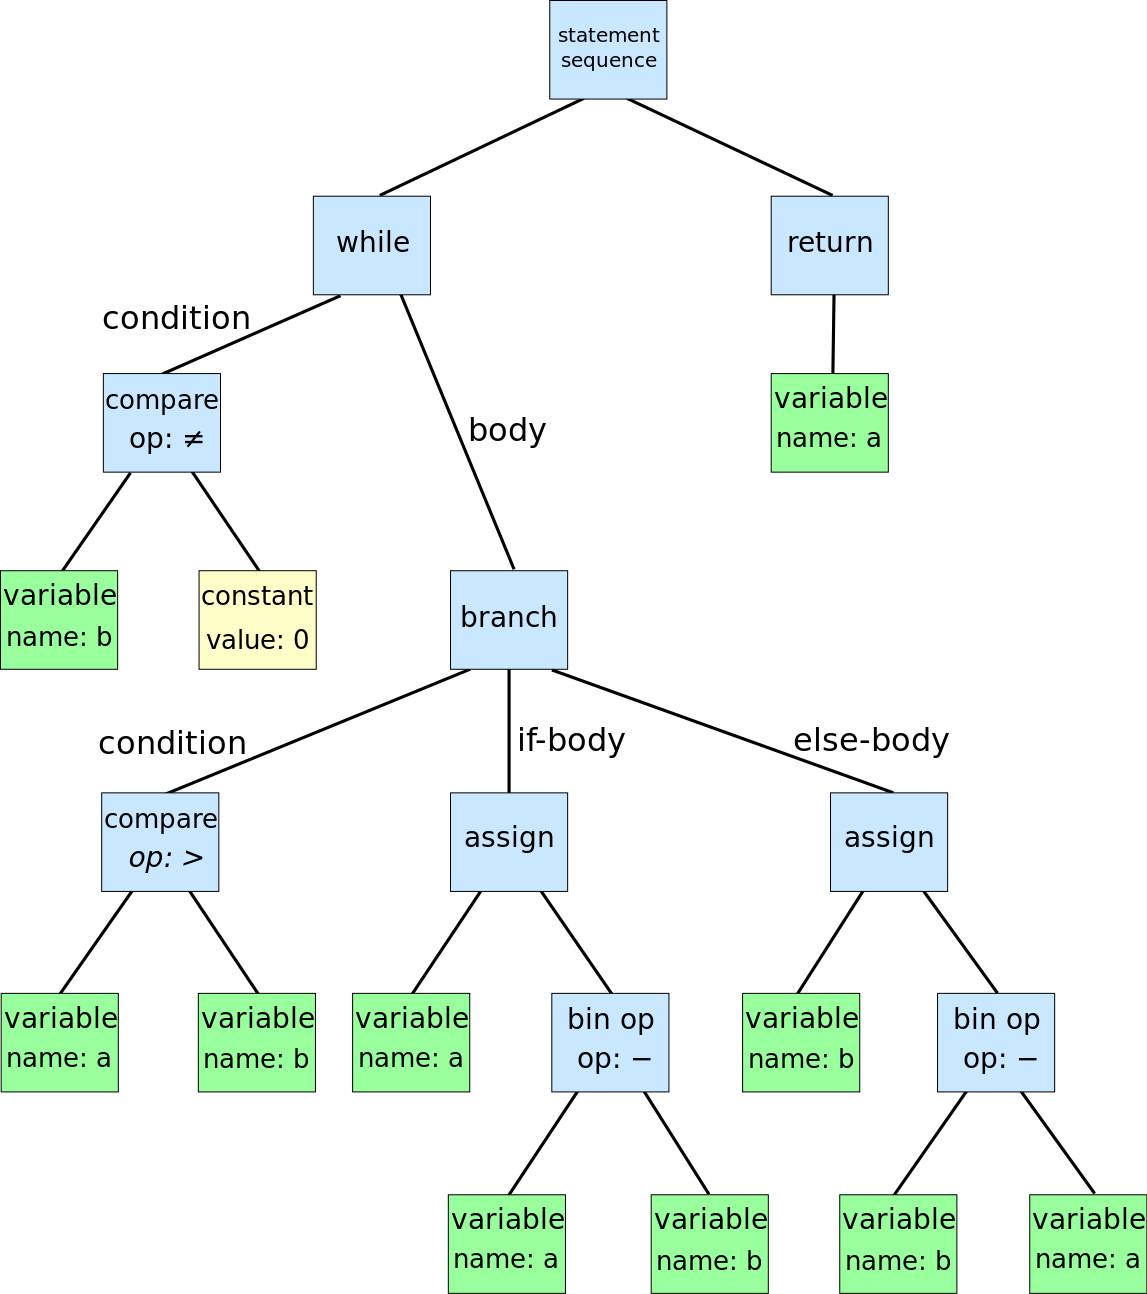
\includegraphics[width = \linewidth]{images/ast.png}
    \end{column}
  \end{columns}
\end{frame}

\begin{frame}{Множественность представлений (2)}
  \centering
  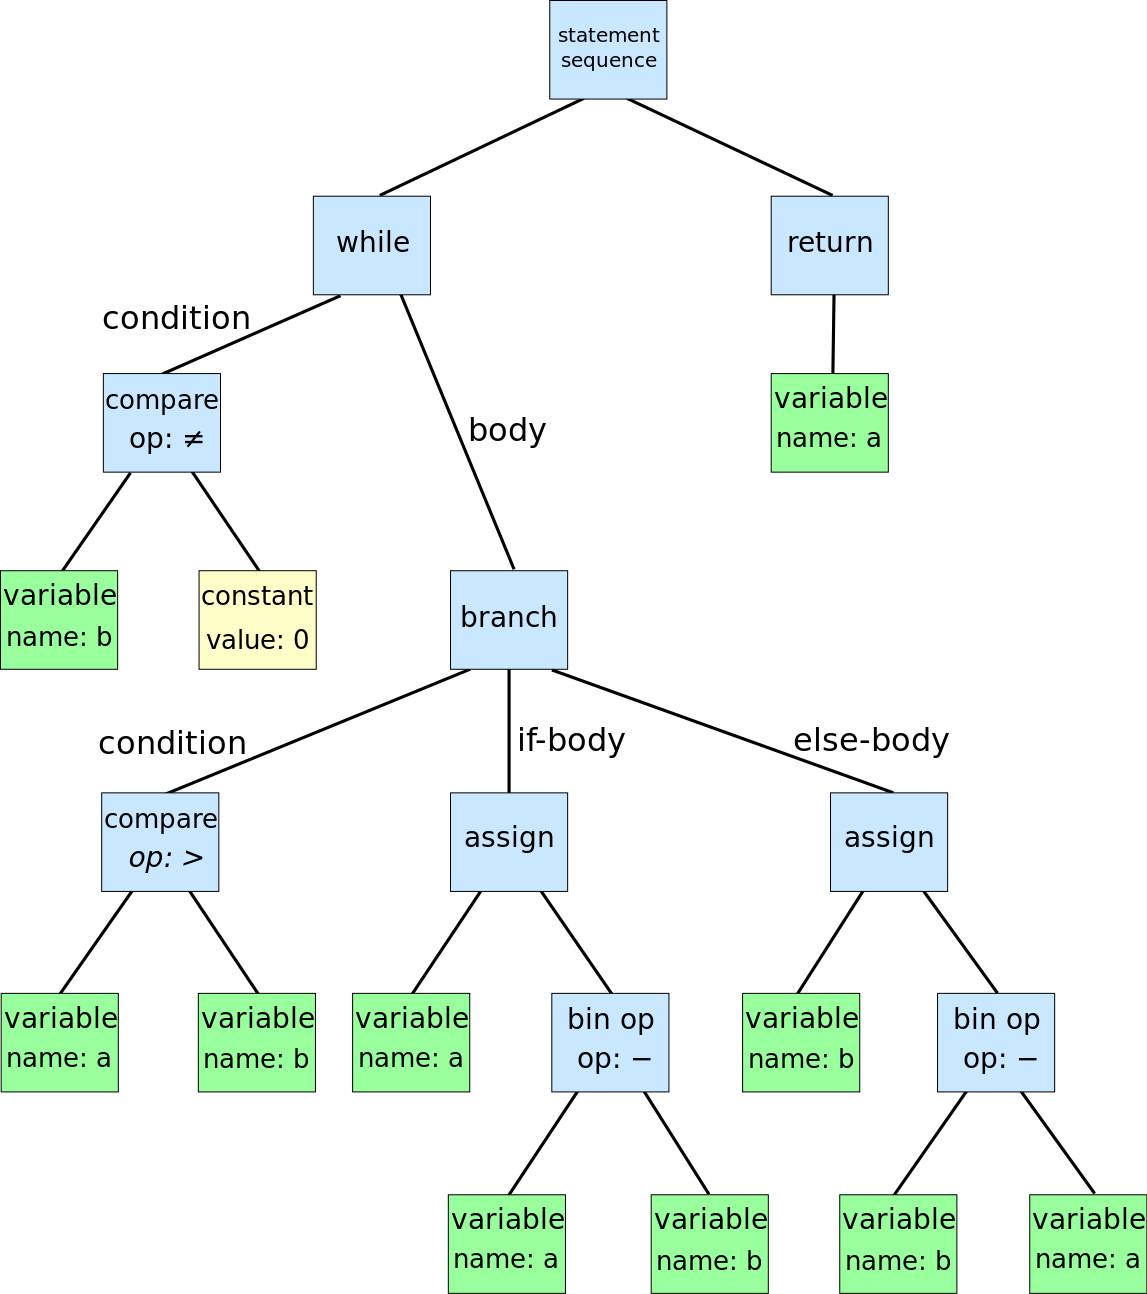
\includegraphics[width = 0.2\linewidth]{images/ast.png}
  \begin{columns}
    \begin{column}{0.3\linewidth}
      \inputminted{c}{codes/ast1.c}
    \end{column}
    \begin{column}{0.5\linewidth}
      \inputminted{c}{codes/ast2.c}
    \end{column}
  \end{columns}
\end{frame}

\begin{frame}{Принтеры (2)}
  \begin{itemize}
    \item Ограничение - ширина вывода
    \item Оценка
      \begin{itemize}
        \item \textcolor{red}{Стиль} \textcolor{gray}{(style guide)}
        \item Наглядность структуры
        \item Обозримость \textcolor{gray}{(размер текста)}
          \begin{itemize}
            \item Оптимальность
          \end{itemize}
      \end{itemize}
  \end{itemize}
\end{frame}

\section{Принтер-комбинаторы}

\begin{frame}{Комбинаторы}
  — это функции высшего порядка, которые из одних функций строят другие
 
	%\vspace{1cm}

  \begin{center}
  \begin{columns}
		\begin{column}{0.5\linewidth}
      \textcolor{myGray}{
        \scriptsize
        %Возможность принимать функции в качестве аргумента и
        %возвращать их в качестве результата —
        %отличительная черта функциональных языков программирования,
        %в которых комбинаторы являются обычными функциями.
        \begin{itemize}
          \item Элементарные функции
          \item Переход от простого к сложному
          \item Пример: парсер-комбинаторы
          \begin{itemize}
            \scriptsize
            \item symbol
            \item >>=
            \item many
            \item option
          \end{itemize}
          \item \textcolor{gray}{Характерны для функционального программирования}
          \item \textcolor{gray}{См. паттерн "Компоновщик" и GUI-frameworks}
        \end{itemize}
      }
		\end{column}
		\begin{column}{0.5\linewidth}
	    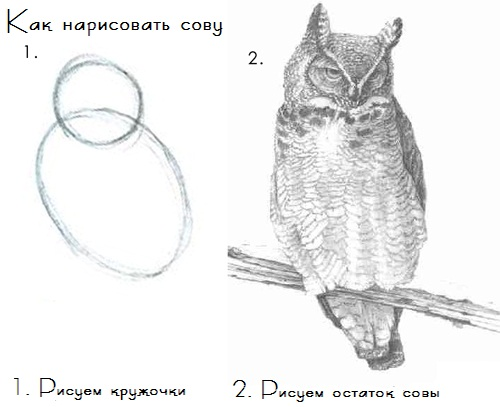
\includegraphics[width = \linewidth]{images/owl.jpg}
		\end{column}
	\end{columns}
  \end{center}
\end{frame}

\begin{frame}{Wadler Doc}
  \inputminted{hs}{codes/wadlerDoc.hs}
\end{frame}

\begin{frame}{Wadler ТТХ}
  \begin{itemize}
    \item Быстро работает \textcolor{gray}{(есть реализации за $O(n)$)}
    \item Не всегда подходит
    \begin{itemize}
      \item Язык Python
        \inputminted{py}{codes/wadlerSeq.py}
    \end{itemize}
  \end{itemize}
\end{frame}

\begin{frame}{Azero, Swierstra Format}
  \inputminted{hs}{codes/swierstraFormat.hs}

  \vspace{0.2cm}

  \begin{columns}
    \begin{column}{0.3\linewidth}
      \centering
      \tikz{
        \draw (0,0) -- (1,0) -- (1,0.2) -- (2,0.2) -- (2,1) -- (0, 1) -- cycle;
      }
    \end{column}
    
    \begin{column}{0.3\linewidth}
      \centering
      \tikz{
        \draw (0,0) -- (1,0) -- (1,0.2) -- (2,0.2) -- (2,1) -- (0, 1) -- cycle;
        \draw (1.1,-0.9) -- (2.1,-0.9) -- (2.1,-0.7) -- (3.1,-0.7) -- (3.1,0.1) -- (1.1,0.1) -- cycle;
      }
    \end{column}

    \begin{column}{0.3\linewidth}
      \centering
      \tikz{
        \draw (0,0) -- (1,0) -- (1,0.2) -- (2,0.2) -- (2,1) -- (0, 1) -- cycle;
        \draw (0,-1.1) -- (1,-1.1) -- (1,-0.9) -- (2,-0.9) -- (2,-0.1) -- (0,-0.1) -- cycle;
      }
    \end{column}
  \end{columns}

  \vspace{0.2cm}

  \begin{columns}
    \begin{column}{0.3\linewidth}
      \centering
      \scriptsize
      Single
    \end{column}
    \begin{column}{0.3\linewidth}
      \centering
      \scriptsize
      Beside
    \end{column}
    \begin{column}{0.3\linewidth}
      \centering
      \scriptsize
      Above
    \end{column}

  \end{columns}
\end{frame}

\begin{frame}{Azero, Swierstra Doc}
  \inputminted{hs}{codes/swierstraDoc.hs}
\end{frame}

\begin{frame}{Azero, Swierstra pretty}
  \inputminted{hs}{codes/swierstraPretty.hs}
\end{frame}

\begin{frame}{Azero, Swierstra ТТХ}
  \begin{itemize}
    \item Работает в худшем случае за $O(2 ^ n)$
    \item Выразительная способность достаточная для применения с шаблонами 
    \item Выдает оптимальный результат
    \begin{itemize}
      \item Самый низкий вариант из попадающих в заданную ширину
    \end{itemize}
  \end{itemize}
\end{frame}

\begin{frame}{BURS}
  Bottom-Up Rewrite Systems

  \begin{itemize}
    \item Динамическое программирование на деревьях (дэгах)
    \item Правила
    $$
    \begin{array}{rcll}

      N &:& \alpha& [c]\\
      N &:& \alpha\; (K_1,\dots,K_n)& [c]
    \end{array}
    $$
    \item Нахождение лучшей раскладки за линейное время от размера структуры
  \end{itemize}

\end{frame}

\begin{frame}{Мои комбинаторы}
  \begin{itemize}
    \item Тот же самый интерфейс и результат,
      
      что и у Azero, Swierstra
    \item Факторизация по размерам Format
      \inputminted{hs}{codes/myCombFS.hs}
    \item Ключ Map - нетерминал в BURS
  \end{itemize}
\end{frame}

\begin{frame}{Алгоритмическая сложность}
  $O(w^{p * k} * n)$
  \begin{itemize}
    \item $k$ - максимальная степень дерева (дэга)
    \item $p$ - размерность ключа Map
    \item $w$ - ширина вывода
    \item В случае комбинаторов Beside, Above, Choice
    \begin{itemize}
      \item $k = 2, p = 2$
      \item Сложность: $O(w^4 * n)$ 
    \end{itemize}

    \item \textcolor{gray}{$w \in 100\dots200$}
    \item \textcolor{gray}{Скоро сложность возрастет до $O(w ^ 6 * n)$ }
 
    % \item Максимальный размер FormatSet: $m = O(w^2)$
    % \item Сложность операций Beside, Above: $O(m^2)$
  \end{itemize}
\end{frame}

\section{Синтаксические шаблоны}

\begin{frame}{Расширение модели комбинаторов (1)}
  Комбинатор Fill
  \vspace{1cm}
  \begin{columns}
    \begin{column}{0.45\linewidth}
        \centering
        \tikz[scale = 1.9]{
          \draw (0,0) -- (1,0) -- (1,0.2) -- (2,0.2) -- (2,1) -- (0, 1) -- cycle;
          \draw (0,-0.1) -- (0,-1.1) -- (1.1,-1.1) -- (1.1,-0.9) -- (2.3,-0.9) -- (2.3, 0.1)
                -- (1.1,0.1) -- (1.1,-0.1) -- cycle;
       }
    \end{column}
    
    \begin{column}{0.45\linewidth}
        \centering
        \tikz[scale = 1.9]{
          \draw (0,0) -- (1,0) -- (1,0.2) -- (2,0.2) -- (2,1) -- (0, 1) -- cycle;
          \draw (0.3,-0.1) -- (0.3,-1.1) -- (1.1,-1.1) -- (1.1,-0.9) -- (2.3,-0.9) -- (2.3, 0.1)
                -- (1.1,0.1) -- (1.1,-0.1) -- cycle;
          \draw[<->] (0,-0.6) -- (0.3,-0.6);
          \draw (0.15,-0.4) node [fill=white] {\tiny fc};
          \draw[dashed] (0,0) -- (0,-1.1);
       }

    \end{column}
  \end{columns}
  
  \vspace{0.3cm}

  \begin{columns}
    \begin{column}{0.45\linewidth}
    \end{column}
    \begin{column}{0.45\linewidth}
        \centering
       {\scriptsize fc - Fill Constant}
    \end{column}
  \end{columns}
\end{frame}

\begin{frame}{Расширение модели комбинаторов (2)}
  Факторизация
  \begin{itemize}
    \item Было : width, lastLineWidth
    \item Стало: width, lastLineWidth, firstLineWidth
  \end{itemize}
  Сложность возрасла до $O(w ^ 6 * n)$

  \vspace{1cm}
  \textcolor{gray}{В таком виде абсолютно не применимо}

\end{frame}

\begin{frame}{Добавление в FormatSet}
  Вводим отношение частичного порядка на Format
  \vspace{1cm}

  Эвристика:
  \begin{itemize}
    \item Добавить только в случае, если нет варианта лучше
    \item Убрать варианты, которые хуже добавляемого
  \end{itemize}
  \vspace{1cm}
  \textcolor{gray}{На данный момент самое критичное по производительности место}
\end{frame}

\begin{frame}{Получение образцов}
\end{frame}

\begin{frame}{Реализация}
  \begin{itemize}
    \item Форматтер-плагин для IDEA
    \item Написан на Kotlin
  \end{itemize}
\end{frame}

\begin{frame}{Нерешенные проблемы}
  \begin{itemize}
    \item Обработка комментариев
      \begin{itemize}
        \item Возможно, шаблоны и для них, т.к. структура известна (JavaDoc, Doxygen) 
      \end{itemize}
    \item Списки (структуры с плавающим числом поддеревьев)
      \begin{itemize}
        \item Сейчас - фиксированное представление
        \item Шаблонный переход от одного элемента к другому
      \end{itemize}
    \item Время работы
      \begin{itemize}
        \item сейчас - 4с
        \item нужно  - 0.5с
      \end{itemize}
  \end{itemize}
\end{frame}

\begin{frame}{Направления развития}
  \begin{itemize}
    \item Абстрагирование от языка
    \item Проверка репозитория шаблонов на полноту
    \item Задание порядка поддеревьев
      \begin{itemize}
        \item Поля, методы, подклассы
      \end{itemize}

    \item Фильтрация 'плохих' шаблонов
    \item Совместное форматирование поддеревьев
  \end{itemize}
\end{frame}

\end{document}
